\documentclass[11pt,a4paper]{article}
\usepackage{fontspec}
\setmainfont{cmunrm.otf}[BoldFont=cmunbx.otf,ItalicFont=cmunti.otf,BoldItalicFont=cmunbi.otf]
\setsansfont{cmunss.otf}[BoldFont=cmunsx.otf]
\setmonofont{cmuntt.otf}
\usepackage[english]{babel}
\usepackage[a4paper,margin=2.3cm]{geometry}
\usepackage{amsmath,amssymb}
\usepackage{graphicx,booktabs,array,tabularx,float}
\usepackage[font=small,labelfont=bf,labelsep=period]{caption}
\usepackage{xcolor,tikz}
\usetikzlibrary{arrows.meta,decorations.markings}
\usepackage[colorlinks,linkcolor=blue!50!black,citecolor=blue!50!black,urlcolor=blue!50!black]{hyperref}
\usepackage{enumitem}
\setlist{itemsep=2pt,topsep=4pt}
\graphicspath{{../figs/en/}}
\linespread{1.08}

\newcommand{\tb}{t_b}
\newcommand{\he}{h/e^2}
\newcommand{\Rxy}{R_{xy}}
\newcommand{\Rxx}{R_{xx}}
\newcommand{\lB}{l_B}
\newcommand{\EF}{E_F}
\newcommand{\hw}{\hbar\omega_c}
\newcommand{\botm}{\text{bot}}
\newcommand{\topp}{\text{top}}

\definecolor{chiral}{HTML}{0b0b0b}
\definecolor{counter}{HTML}{eb6834}
\definecolor{pocket}{HTML}{2a78d6}

\title{Counter-propagating edge channels in a pocket\\ of the confining
potential and the Hall response\\[4pt]
\large a numerical study}
\author{Working note}
\date{29 September 2026}

\begin{document}
\maketitle

\begin{abstract}
\noindent
We study numerically (Kwant, tight-binding model) a six-terminal Hall bar
whose confining potential forms a well (a ``pocket'') in front of the edge.
Inside the pocket the next Landau level crosses the Fermi energy twice, and
a pair of edge channels appears, one of which runs against the chirality.
Everything that happens to such a pair between two neighbouring contacts
reduces to a single number, the backward transmission probability $\tb$,
which gives the Hall and longitudinal resistances explicitly. Quantization
is broken when the counter-propagating channel reaches a contact
($\tb\neq0$). Backscattering inside the pair restores it. With the
image-charge potential of Ref.~\cite{andolina} the picture is the same. The
two-terminal conductance on which the conclusions of~\cite{andolina} rest
equals $\nu+\tb$. It is therefore an integer both for $\tb=0$ and for
$\tb=1$, and it misses exactly the regime in which the Hall bar deviates
most. We end with signatures of the mechanism that can be tested in a
four-terminal geometry.
\end{abstract}

\tableofcontents

%======================================================================
\section{The question}

In experiments with a GaAs two-dimensional electron gas placed inside a
metallic split-ring resonator, the plateaus of the quantum Hall effect were
found to be distorted~\cite{appugliese}. This was first attributed to the
vacuum fluctuations of the resonator field. Ref.~\cite{andolina} proposes an
electrostatic explanation instead. The metal of the resonator next to the
mesa edge carries the image of the electron, which pulls the electron
towards the edge. Together with a steep confining potential this produces a
well at the edge that hosts counter-propagating (non-chiral) edge channels.
The authors of~\cite{andolina} compute only the two-terminal conductance
$G(\EF)$. The comment~\cite{ciuti} objects that (i)~the self-consistent
electrostatics of a GaAs mesa does not produce a pocket, and (ii)~the
experiment measures $\Rxx$ and $\Rxy$ in a Hall bar, not a two-terminal
conductance.

We do not address whether the pocket exists (point~(i)): here the pocket is
put in by hand. We ask \emph{what it does to the Hall response if it does
exist}:
\begin{enumerate}
\item does a counter-propagating channel on one edge spoil $\Rxy$ and
      $\Rxx$ of a six-terminal Hall bar;
\item under which conditions (overlap of the partners, disorder, contact
      geometry);
\item how this compares with the conclusions of~\cite{andolina}, which are
      drawn from the two-terminal conductance.
\end{enumerate}
The resonator as a dynamical system is not considered.

%======================================================================
\section{Model}

\subsection{Hamiltonian and units}
Square lattice with lattice constant $a=1$ and hopping $t=1$:
\begin{equation}
H=\sum_i\bigl(4t+V_i\bigr)c_i^\dagger c_i-t\sum_{\langle ij\rangle}
e^{i\theta_{ij}}c_i^\dagger c_j,
\end{equation}
where the Peierls phases $\theta_{ij}$ correspond to a flux of $\varphi$
flux quanta $h/e$ per plaquette. In the continuum limit
$\hw\simeq4\pi\varphi\,t$ and $\lB=a/\sqrt{2\pi\varphi}$.
Unless stated otherwise the Fermi energy is fixed at $\EF=0.4\,t$ and the
field is swept over $\varphi=0.008\ldots0.06$ (plateaus $\nu=4\ldots1$,
$\lB\approx1.6\ldots4.5\,a$). The field calibration was checked against the
Landau level spacing of a ribbon in the Landau gauge and against the
plateau positions.

\subsection{Geometry}
A $300\times80$ bar with four probes of width $56$ (much wider than the
pocket and $\lB$) and six ideal ohmic contacts: semi-infinite leads in the
same field and with the same edge profile (Fig.~\ref{fig:scheme}). Current
flows $0\to3$; probes 1, 2, 4, 5 are floating. For our sign of the field,
electrons go around the perimeter as $0\to5\to4\to3\to2\to1\to0$.

\begin{figure}[ht]
\centering
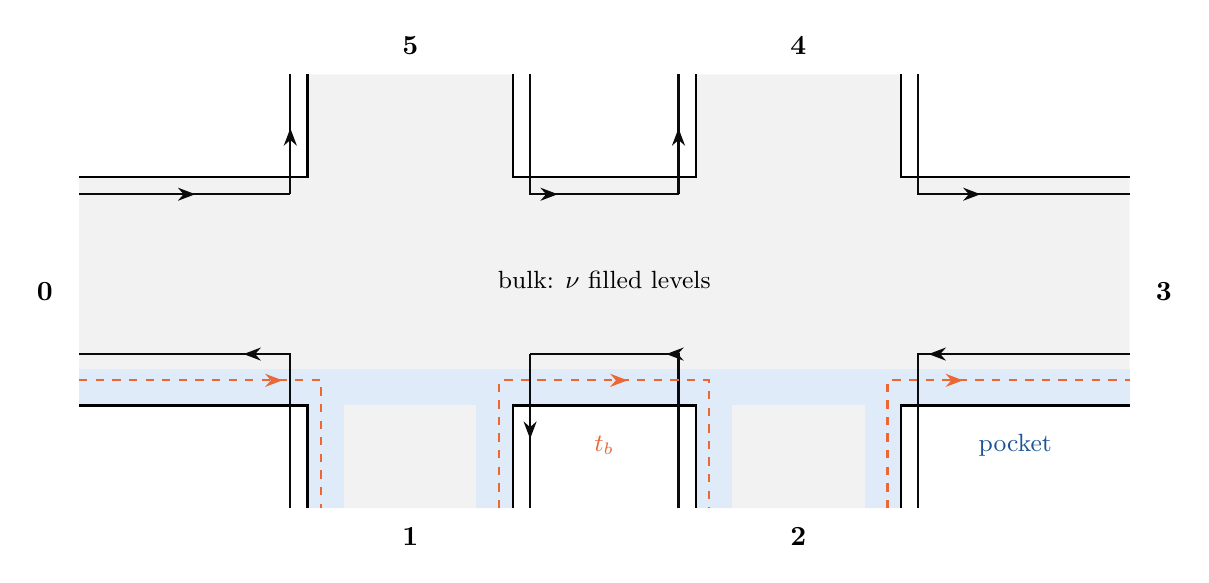
\begin{tikzpicture}[x=1.45cm,y=1.45cm,
  chir/.style={chiral,thick,decoration={markings,mark=at position 0.55 with {\arrow{Stealth[length=2.2mm]}}},postaction=decorate},
  ctr/.style={counter,thick,dashed,decoration={markings,mark=at position 0.55 with {\arrow{Stealth[length=2.2mm]}}},postaction=decorate}]
  % sample
  \fill[black!5] (-0.6,0) -- (1.4,0) -- (1.4,-0.9) -- (3.2,-0.9) -- (3.2,0) -- (4.8,0) -- (4.8,-0.9)
    -- (6.6,-0.9) -- (6.6,0) -- (8.6,0) -- (8.6,2) -- (6.6,2) -- (6.6,2.9) -- (4.8,2.9) -- (4.8,2)
    -- (3.2,2) -- (3.2,2.9) -- (1.4,2.9) -- (1.4,2) -- (-0.6,2) -- cycle;
  % pocket band along the bottom edge
  \fill[pocket!15] (-0.6,0) rectangle (8.6,0.32);
  \fill[pocket!15] (1.4,-0.9) rectangle (1.72,0); \fill[pocket!15] (2.88,-0.9) rectangle (3.2,0);
  \fill[pocket!15] (4.8,-0.9) rectangle (5.12,0); \fill[pocket!15] (6.28,-0.9) rectangle (6.6,0);
  % outline
  \draw[thick] (-0.6,0) -- (1.4,0) -- (1.4,-0.9) (3.2,-0.9) -- (3.2,0) -- (4.8,0) -- (4.8,-0.9)
               (6.6,-0.9) -- (6.6,0) -- (8.6,0);
  \draw[thick] (-0.6,2) -- (1.4,2) -- (1.4,2.9) (3.2,2.9) -- (3.2,2) -- (4.8,2) -- (4.8,2.9)
               (6.6,2.9) -- (6.6,2) -- (8.6,2);
  % contacts
  \foreach \x/\y/\n in {-0.9/1/0, 8.9/1/3, 2.3/-1.15/1, 5.7/-1.15/2, 5.7/3.15/4, 2.3/3.15/5}
    \node[font=\bfseries] at (\x,\y) {\n};
  % chiral channels
  \draw[chir] (-0.6,1.85) -- (1.25,1.85);
  \draw[chir] (1.25,1.85) -- (1.25,2.9);
  \draw[chir] (3.35,2.9) -- (3.35,1.85) -- (4.65,1.85);
  \draw[chir] (4.65,1.85) -- (4.65,2.9);
  \draw[chir] (6.75,2.9) -- (6.75,1.85) -- (8.6,1.85);
  \draw[chir] (8.6,0.45) -- (6.75,0.45) -- (6.75,-0.9);
  \draw[chir] (4.65,-0.9) -- (4.65,0.45) -- (3.35,0.45);
  \draw[chir] (3.35,0.45) -- (3.35,-0.9);
  \draw[chir] (1.25,-0.9) -- (1.25,0.45) -- (-0.6,0.45);
  % counter-propagating channel in the pocket
  \draw[ctr] (-0.6,0.22) -- (1.52,0.22) -- (1.52,-0.9);
  \draw[ctr] (3.08,-0.9) -- (3.08,0.22) -- (4.92,0.22) -- (4.92,-0.9);
  \draw[ctr] (6.48,-0.9) -- (6.48,0.22) -- (8.6,0.22);
  \node[counter,font=\small] at (4,-0.35) {$\tb$};
  \node[font=\small,align=center] at (4,1.1) {bulk: $\nu$ filled levels};
  \node[pocket!70!black,font=\small] at (7.6,-0.35) {pocket};
\end{tikzpicture}
\caption{The Hall bar. Black arrows: the $\nu$ chiral channels on each edge
(one is drawn). Blue band: the pocket at the bottom edge (including the
bottom probes and the lower halves of leads 0 and~3). Orange dashes: the
counter-propagating channel at the inner border of the pocket; its
co-propagating partner at the outer border is not drawn. $\tb$ is the
probability that an electron emitted by the downstream contact reaches the
upstream contact against the chirality.}
\label{fig:scheme}
\end{figure}

\subsection{Edge profile}
The potential depends on the distance $d$ to the sample boundary. The wall
is smooth:
\[
V_\text{wall}(d)=V_w\Bigl(\frac{d_0-d}{d_0}\Bigr)^2\theta(d_0-d),\qquad
V_w=1.5\,t,\ d_0=6\,a .
\]
We consider two kinds of pocket.
\begin{itemize}
\item \textbf{Rectangular pocket} (Sec.~\ref{sec:rect}):
  $V(d)=V_\text{wall}(d)-V_\text{dip}\,w(d;d_\text{in},d_\text{out})$, where
  $w$ is a smoothed window ($\tanh$ fronts of width $a$) and
  $d_\text{in}=6$. \emph{Wide} pocket: $V_\text{dip}=0.3\,t$, width $14\,a$;
  the pair is separated by $\approx5.8\,\lB$ (at $\nu=1$, $\varphi=0.028$)
  with overlap $<0.01$. \emph{Narrow} pocket: $V_\text{dip}=0.35\,t$, width
  $4\,a$; separation $\approx1.6\,\lB$, overlap $\approx0.57$.
\item \textbf{Image-charge potential} (Sec.~\ref{sec:image}), in the form
  of~\cite{andolina}: a metal plate parallel to the edge at distance
  $d_\text{edge}$,
  \begin{equation}\label{eq:img}
  V(d)=V_\text{wall}(d)-E_\text{img}\Bigl[\frac1{d+d_\text{edge}}-
  \frac1{d_c+d_\text{edge}}\Bigr]\theta(d_c-d),
  \end{equation}
  with $d_c=40\,a$ (the middle of the bar), so that the bulk and the
  opposite edge are untouched.
\end{itemize}
The overlap of the partners is defined as $O=\sum_y|\psi_1(y)||\psi_2(y)|$
($1$ for identical, $0$ for disjoint mode wave functions of an infinite
ribbon with the same profile).

Placements of the pocket: bottom edge only; both edges; and a \emph{local}
pocket on the bottom edge between probes 1 and 2 that does not touch any
contact. Anderson disorder $U=1\,t$ (uniform in $[-U/2,U/2]$) fills the
whole scattering region; ``clean'' runs have $U=0$.

\subsection{Observables}
From the Kwant~\cite{kwant} scattering matrix we build the conductance
matrix $G_{ij}$, drive a current $I$ from contact 0 to contact 3 (grounded)
and solve for the potentials of the floating probes. Then (all resistances
in units of $\he$)
\[
\Rxy^{(1\text{--}5)}=\frac{V_5-V_1}{I},\quad
\Rxy^{(2\text{--}4)}=\frac{V_4-V_2}{I},\quad
\Rxx^{\botm}=\frac{V_1-V_2}{I},\quad
\Rxx^{\topp}=\frac{V_5-V_4}{I},\quad
R_\text{2t}=\frac{V_0-V_3}{I}.
\]
For the comparison with~\cite{andolina} we also compute the two-terminal
conductance $G_\text{2t}$ of a plain $300\times80$ bar without probes and
with the same edge profile.

%======================================================================
\section{Where the counter-propagating channel comes from}

For a potential that is smooth on the scale of $\lB$, the Landau levels
follow it, $E_n(y)\approx\hw(n+\tfrac12)+V(y)$, and the group velocity
along the edge is proportional to $\partial_yV$. Let $\EF$ lie between
levels $n$ and $n+1$ in the bulk. If level $n+1$ dips below $\EF$ inside
the pocket, it crosses $\EF$ twice. The outer crossing (on the wall side)
gives a channel co-propagating with the chiral ones. The inner crossing,
where $\partial_yV$ has the opposite sign, gives a
\emph{counter-propagating} channel. This happens on the low-field side of
every plateau, as long as $(n+\tfrac32)\hw-V_\text{dip,eff}<\EF$
(Fig.~\ref{fig:edge}). A narrow pocket gives a pair about $\lB$ apart, a
wide pocket a well-separated pair.

\begin{figure}[ht]
\centering
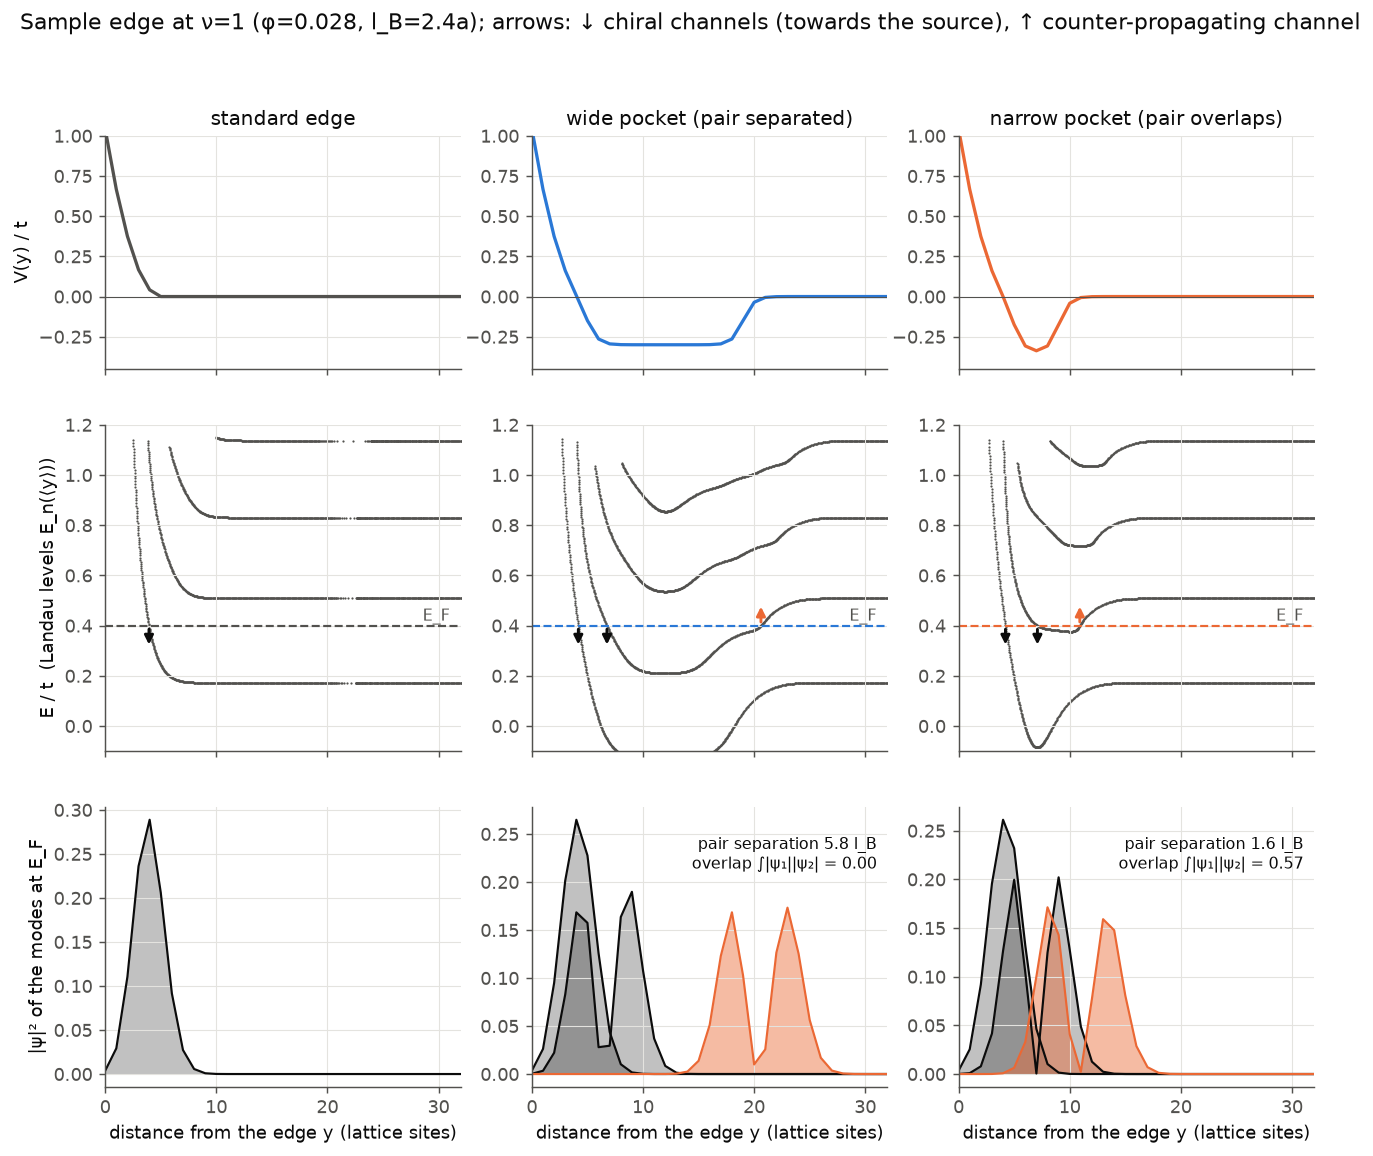
\includegraphics[width=\textwidth]{fig1_edge_structure.png}
\caption{The edge at $\nu=1$ ($\varphi=0.028$). Top to bottom: the
potential profile; ribbon eigenenergies against the position of the state
$\langle y\rangle$ (bent Landau levels), with arrows marking the modes at
$\EF$ (black: chiral, orange: counter-propagating); profiles of the modes at
$\EF$. Left to right: standard edge, wide and narrow pockets.}
\label{fig:edge}
\end{figure}

%======================================================================
\section{The general statement: a single parameter $\tb$}\label{sec:lb}

\subsection{An edge segment}
Consider a piece of the edge between neighbouring contacts $a$ (upstream)
and $b$ (downstream). It carries $\nu$ chiral channels and the pair
(co-propagating + counter-propagating). Contact $a$ sends $\nu+1$ channels
into the segment and receives one (the counter-propagating channel);
contact $b$ sends one channel into the segment and receives $\nu+1$. If no
current leaks through the bulk to other contacts, unitarity of the segment
scattering matrix gives
\[
T_{a\leftarrow b}+R_{b}=1,\qquad T_{b\leftarrow a}+R_{b}=\nu+1
\quad\Longrightarrow\quad
T_{b\leftarrow a}-T_{a\leftarrow b}=\nu .
\]
Whatever the scattering inside the segment is (elastic backscattering,
channel mixing, partial equilibration), the segment is fully described by
one number, the \emph{backward transmission}
$\tb\equiv T_{a\leftarrow b}\in[0,1]$. $\tb=0$ is a perfect quantum Hall
edge; $\tb=1$ is a ballistic counter-propagating channel.

\subsection{Formulas for the Hall bar}
For a pocket on the bottom edge with the same $\tb$ on all three bottom
segments, the Landauer--Büttiker equations~\cite{buttiker} can be solved in
closed form (Table~\ref{tab:lb}).

\begin{table}[ht]
\centering
\caption{Resistances of the Hall bar with a pocket on the bottom edge (in
$\he$).}
\label{tab:lb}
\begin{tabular}{lcc}
\toprule
quantity & formula & $\nu=1,\ \tb=1$\\
\midrule
$\Rxy^{(1\text{--}5)}$ & $1/(\nu+\tb)$ & $1/2$\\
$\Rxy^{(2\text{--}4)}$ & $(\nu+2\tb)/(\nu+\tb)^2$ & $3/4$\\
$\Rxx^\botm$ & $\tb/(\nu+\tb)^2$ & $1/4$\\
$\Rxx^\topp$ & $0$ & $0$\\
$R_\text{2t}$ (with floating probes) & $(\nu^2+3\nu\tb+3\tb^2)/(\nu+\tb)^3$ & $7/8$\\
\bottomrule
\end{tabular}
\end{table}

For a plain two-terminal bar whose leads carry the same edge,
\begin{equation}\label{eq:g2t}
G_\text{2t}=\nu+\tb^{\text{(full length)}}\quad[e^2/h],
\end{equation}
where $\tb$ is taken over the whole length of the edge from drain to source.

\subsection{Consequences}
\begin{itemize}
\item \textbf{Quantization is broken by the absence of backscattering, not
  by backscattering.} A ballistic counter-propagating channel ($\tb=1$)
  carries the potential of the downstream contact back to the upstream one.
  This shifts $\Rxy$ and gives $\Rxx\neq0$ without any dissipation in the
  bulk; the bulk $\sigma_{xy}=\nu e^2/h$ stays topological.
\item \textbf{Backscattering inside the pair heals.} If the partners
  overlap and disorder backscatters electrons, the counter-propagating
  channel localizes along the edge, $\tb\sim e^{-L/\xi}\to0$, and
  quantization is restored.
\item \textbf{A contact is needed.} If the pocket is local and does not
  touch any ohmic contact, the pair forms a closed loop, $\tb\equiv0$, and
  there is no effect in DC transport.
\item The edge without a pocket stays ideal ($\Rxx^\topp=0$), and the
  difference of the two Hall voltages equals exactly $\Rxx$ of the
  defective edge.
\end{itemize}

%======================================================================
\section{Rectangular pocket}\label{sec:rect}

\subsection{Pocket on one (bottom) edge}
In Fig.~\ref{fig:sweeps} the grey curves are the standard sample: plateaus
$\Rxy=h/\nu e^2$ and $\Rxx=0$, with the mesoscopic fluctuations typical of a
small coherent sample between the plateaus. The curves are averaged over
three disorder realizations.

\begin{figure}[ht]
\centering
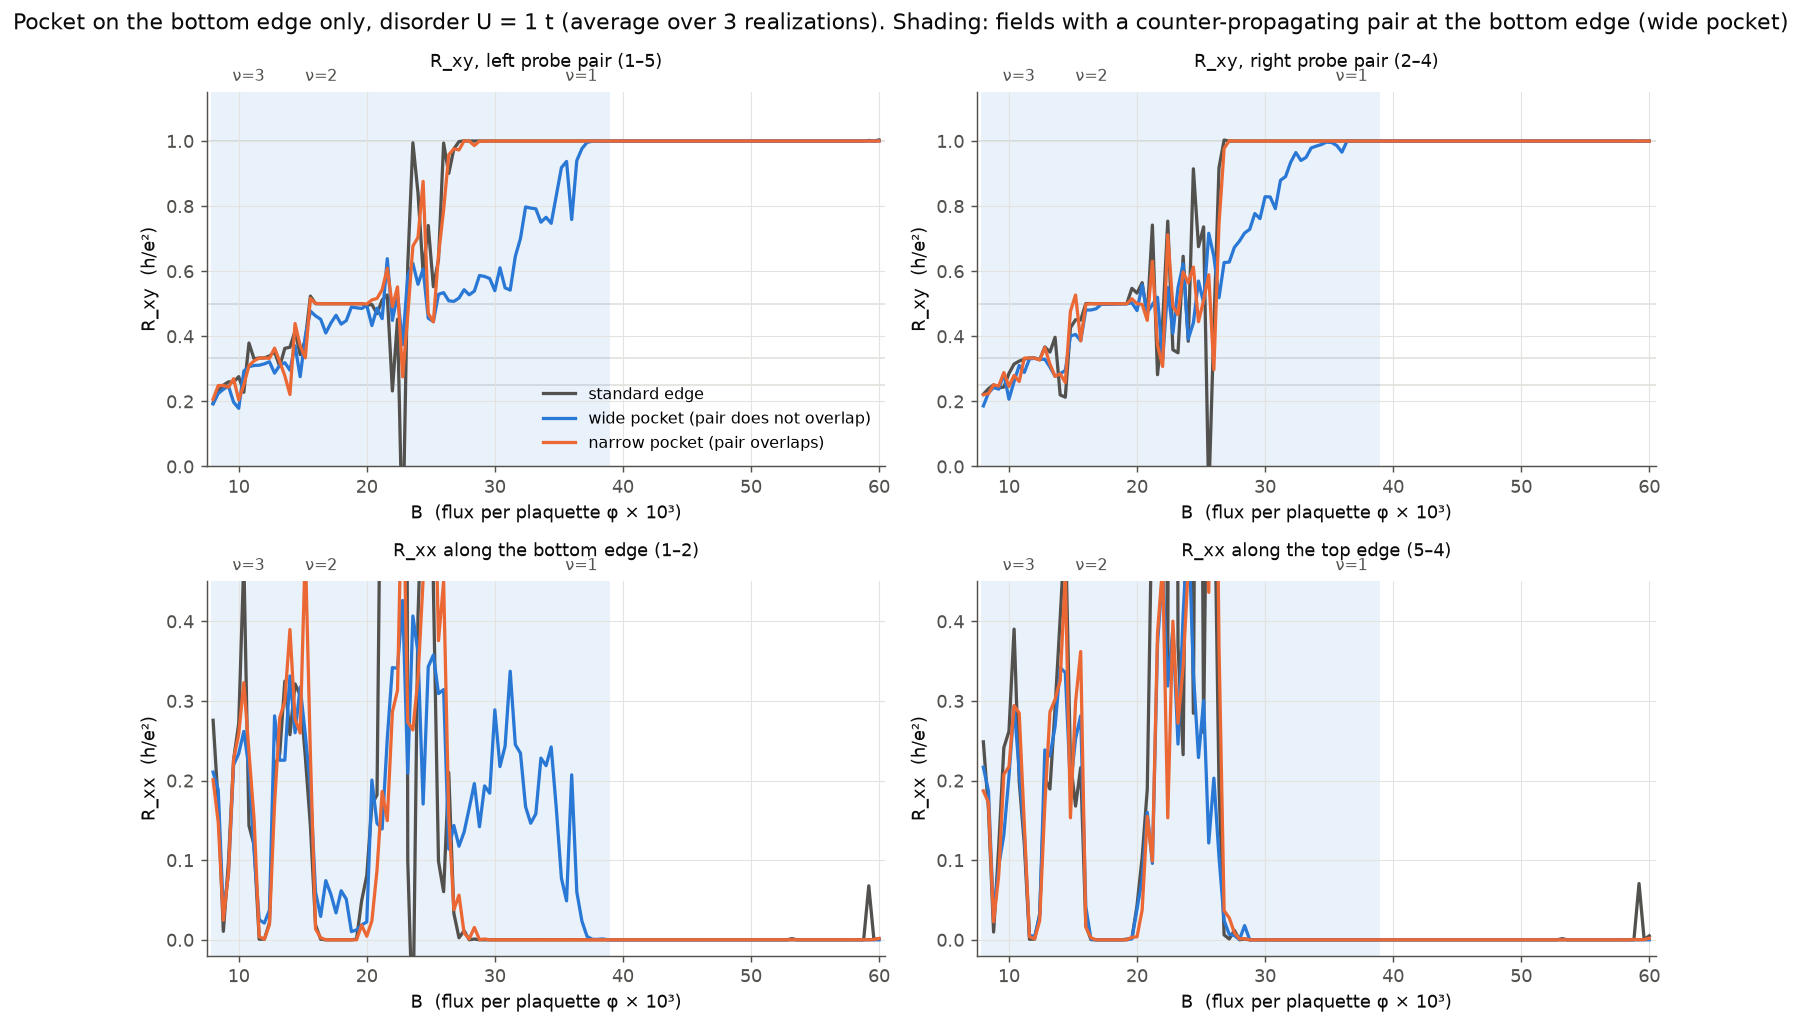
\includegraphics[width=\textwidth]{fig2_sweeps_bottom_pocket.png}
\caption{Field sweep at $\EF=0.4\,t$, $U=1\,t$, averaged over three
realizations. Shading: fields at which the bottom edge carries a
counter-propagating pair (wide pocket).}
\label{fig:sweeps}
\end{figure}

\begin{itemize}
\item \textbf{Wide pocket} (pair separated by 4--6~$\lB$): on the low-field
  part of the $\nu=1$ plateau ($\varphi\approx0.027$--$0.038$)
  $\Rxy^{(1\text{--}5)}$ drops to 0.51--0.60 (at
  $\varphi\approx0.027$--$0.031$; further on the deviation gradually
  shrinks), and $\Rxy^{(2\text{--}4)}$ drops to $\approx0.63$.
  $\Rxx^\botm$ reaches $\approx0.34$, while $\Rxx^\topp=0$ to within
  $10^{-4}$ at $\varphi>0.03$. The same, weaker, is seen on the $\nu=2$
  plateau. At $\varphi>0.039$ there is no pair and the curves coincide with
  the reference.
\item \textbf{Narrow pocket} (separation $\approx1.6\,\lB$, overlap
  $\approx0.6$): the pair exists at $\varphi\approx0.022$--$0.029$, partly
  inside the $2\to1$ transition. On the plateau part
  $\varphi\approx0.0275$--$0.0285$ disorder brings $\Rxy$ back to $\he$
  within $\le0.015$, whereas without disorder $\Rxy^{(1\text{--}5)}=0.50$--$0.54$
  there (Fig.~\ref{fig:clean}).
\end{itemize}

\subsection{Clean versus disordered}
Without disorder the counter-propagating channel is ballistic, $\tb=1$, and
Kwant reproduces Table~\ref{tab:lb} \emph{exactly}:
$\Rxy^{(1\text{--}5)}=1/(\nu+1)$ ($0.5$; $0.333$; $0.25$ for $\nu=1,2,3$),
$\Rxy^{(2\text{--}4)}=(\nu+2)/(\nu+1)^2$ ($0.75$; $0.444$; $0.3125$),
$\Rxx^\botm=1/(\nu+1)^2$ ($0.25$; $0.111$; $0.0625$), over the whole field
range where the pair exists. This holds \emph{for the narrow pocket too}:
without scatterers the pair by itself, even an overlapping one, gives the
maximal deviation. Switching on disorder in the narrow pocket restores exact
quantization (Fig.~\ref{fig:clean}).

\begin{figure}[ht]
\centering
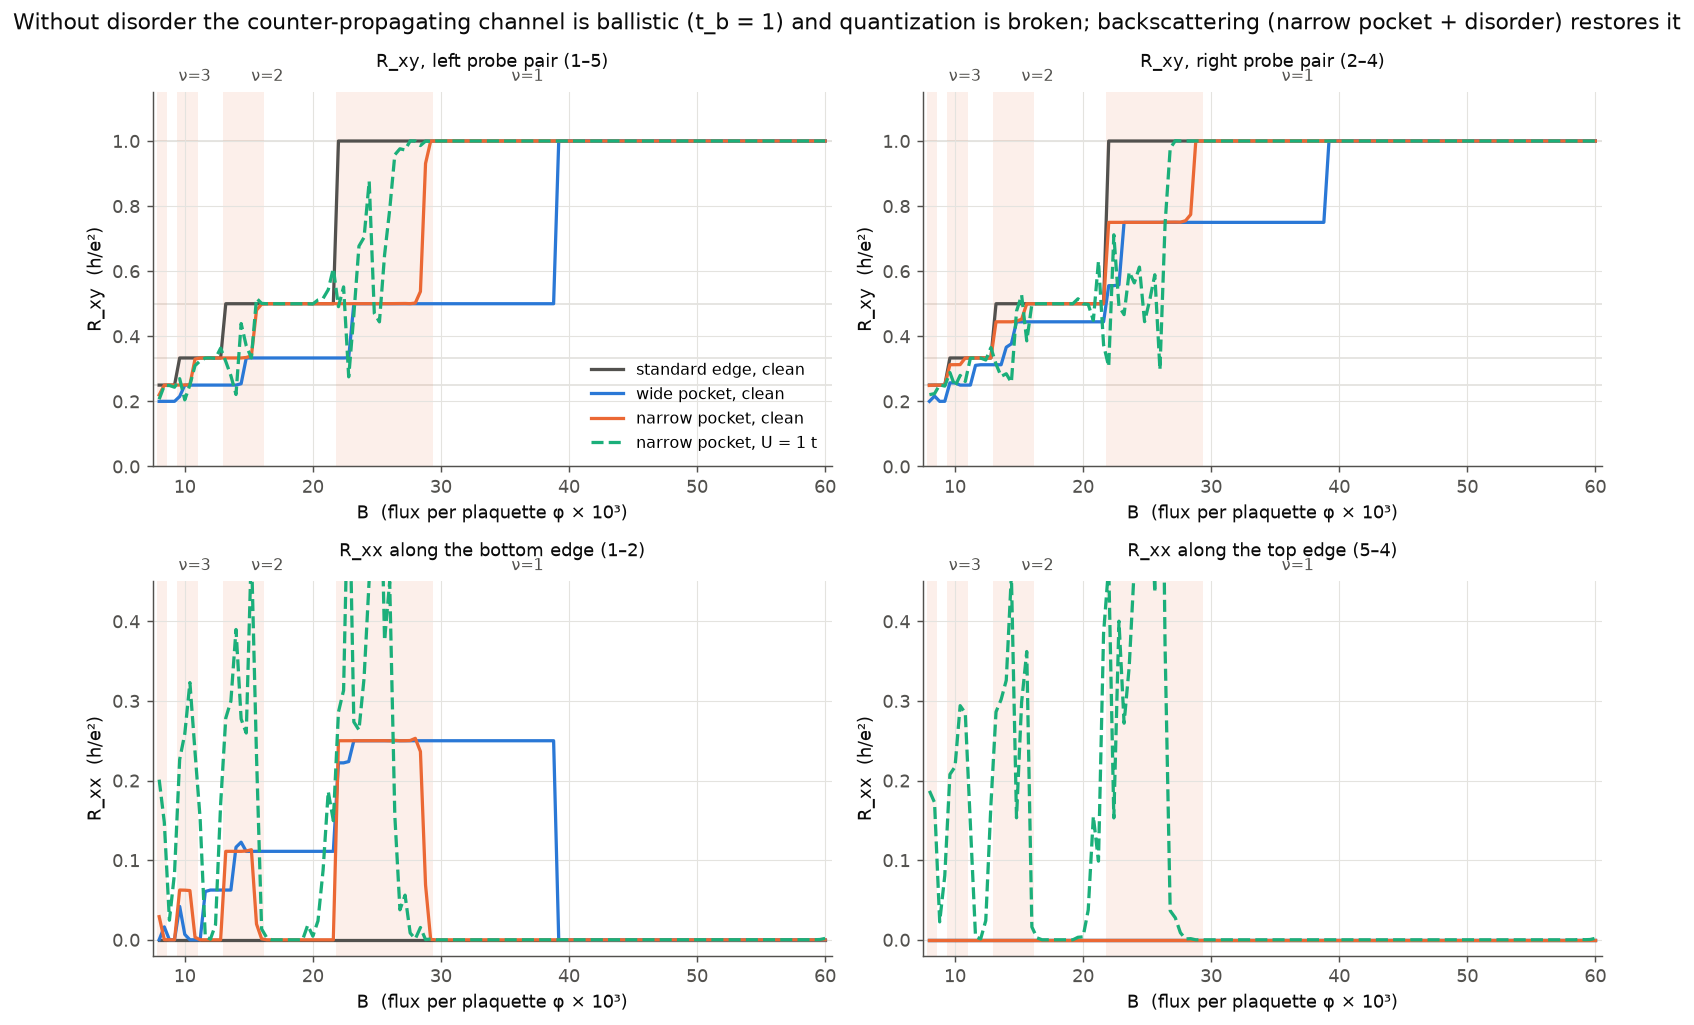
\includegraphics[width=\textwidth]{fig3_clean_vs_disorder.png}
\caption{Without disorder ($\tb=1$) quantization is broken according to
Table~\ref{tab:lb}; backscattering (narrow pocket + disorder, green dashed
line) restores it.}
\label{fig:clean}
\end{figure}

Fig.~\ref{fig:tb} shows on the left $\tb$ between probes 1 and 2, taken
directly from the scattering matrix, and on the right the formulas of
Table~\ref{tab:lb} together with Kwant points on the plateaus. In the wide
pocket with disorder part of the counter-propagating flow bypasses a probe
(for example $0\to2$ bypassing probe 1, with probability up to $\approx0.3$),
so the single-$\tb$ formula is only approximate there. All curves in the
figures are computed from the full transmission matrix, not from this
formula.

\begin{figure}[ht]
\centering
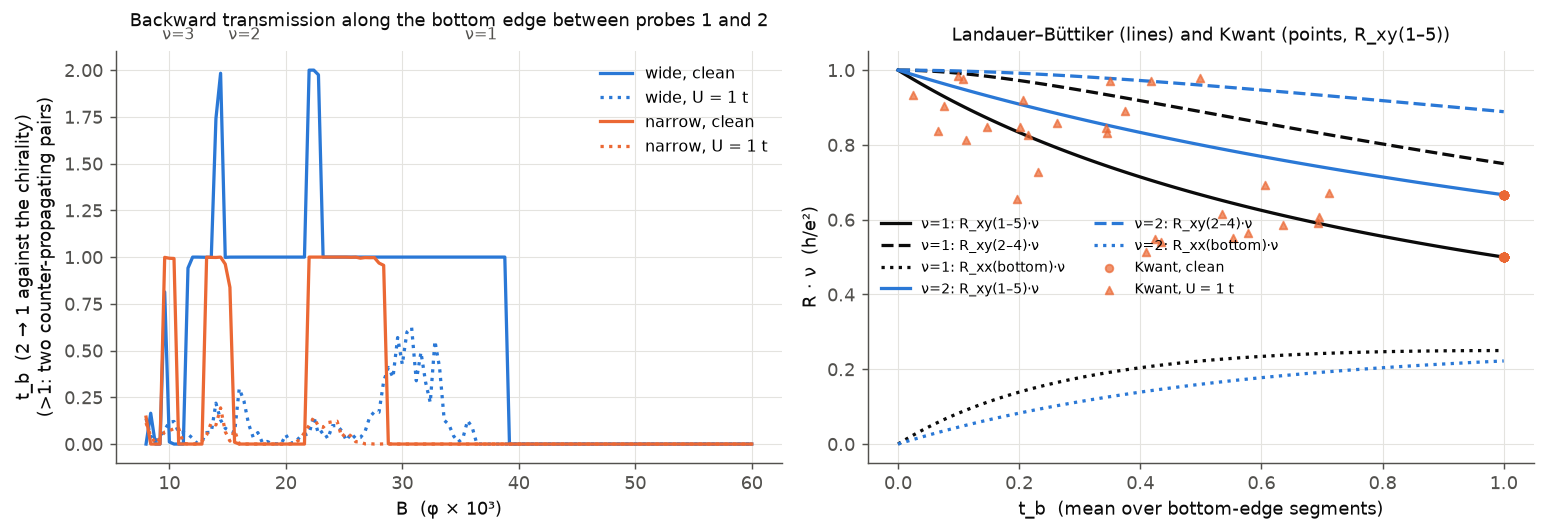
\includegraphics[width=\textwidth]{fig5_tb_and_LB.png}
\caption{Left: backward transmission $\tb$ along the bottom edge between
probes 1 and~2. Right: Landauer--Büttiker formulas (lines) and Kwant
(points, $\Rxy^{(1\text{--}5)}$).}
\label{fig:tb}
\end{figure}

\subsection{Do the partners overlap? The pocket width}
At fixed field ($\nu=1$, $\varphi=0.028$), pocket depth $0.35\,t$ and
$U=1\,t$ (three realizations) we vary only the pocket width, i.e.\ the
distance between the counter-propagating channels (Fig.~\ref{fig:width},
Table~\ref{tab:width}). While the partners overlap, disorder backscatters
electrons within the pair, the counter-propagating channel localizes on a
length shorter than the distance between contacts, and the response is
quantized. Once the partners are separated, there is no backscattering, the
counter-propagating channel reaches a contact, and quantization is broken.

\begin{table}[ht]
\centering
\caption{Dependence on the pair separation ($\nu=1$, average over three
realizations).}
\label{tab:width}
\begin{tabular}{lcccc}
\toprule
pair separation & $\le2.3\,\lB$ & $2.7\,\lB$ & $3.5\,\lB$ & $\ge4.3\,\lB$\\
\midrule
overlap $O$ & 0.9--0.5 & 0.43 & 0.20 & $\le0.06$\\
$\tb$ (segment 1--2) & $\approx0$--0.01 & 0.03 & 0.18 & 0.2--0.4\\
$\Rxy^{(1\text{--}5)}$, $\he$ & 0.97--1.00 & 0.94 & 0.75 & 0.53--0.58\\
$\Rxx^\botm$, $\he$ & $\le0.03$ & 0.06 & 0.19 & 0.15--0.27\\
\bottomrule
\end{tabular}
\end{table}

\begin{figure}[ht]
\centering
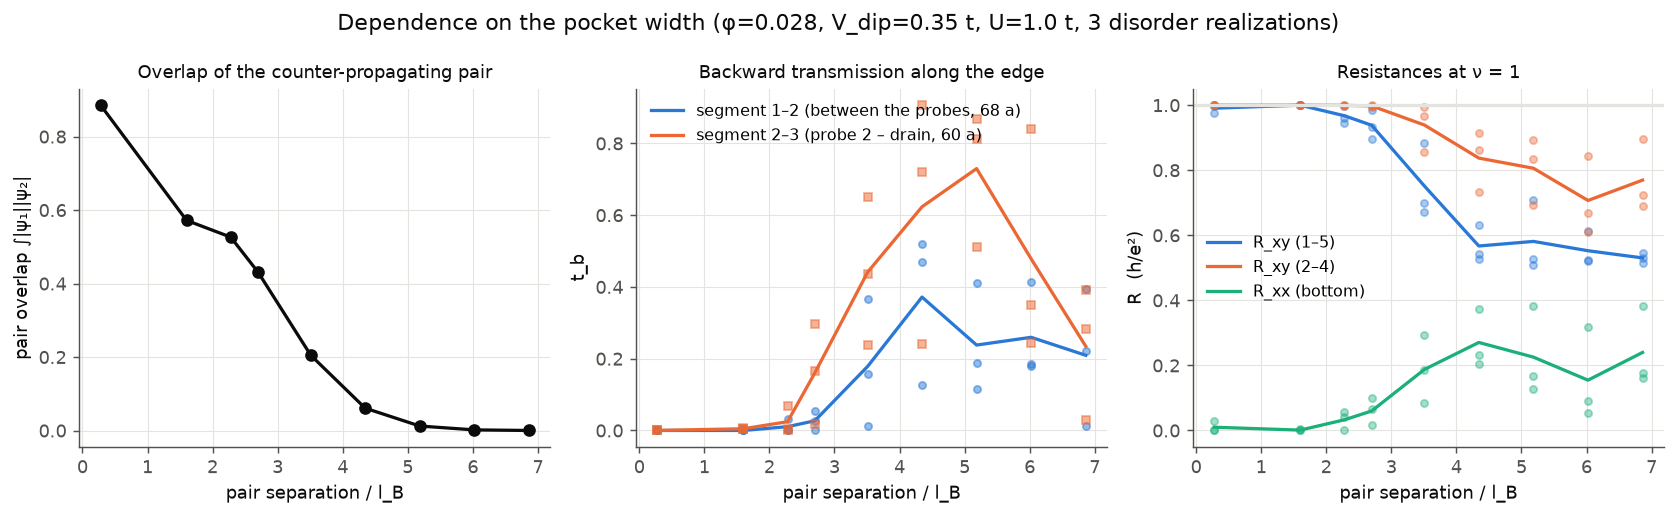
\includegraphics[width=\textwidth]{fig6_width_sweep.png}
\caption{Dependence on the pocket width: pair overlap, backward
transmission along two bottom-edge segments, and resistances at $\nu=1$.
Points: individual disorder realizations; lines: averages.}
\label{fig:width}
\end{figure}

\subsection{Pockets on both edges and a local pocket}
\begin{itemize}
\item Wide pockets on both edges: the deviations add up. For a ballistic
  pair the Landauer--Büttiker formulas give $\Rxy=1/3$, $\Rxx=2/9$ at
  $\nu=1$; Kwant with disorder gives $\Rxy\approx0.36$--$0.48$ on the
  low-field part of the plateau ($\varphi\approx0.027$--$0.031$), rising
  towards 1 at higher field.
\item Narrow pockets on both edges with disorder: quantization survives,
  $|\Rxy-\he|\le3\cdot10^{-3}$ on the $\nu=1$ plateau (one realization).
\item A wide pocket only on the part of the bottom edge between probes 1
  and 2, reaching no contact: the pair is closed into a loop, $\tb\equiv0$,
  and on the plateaus the curves coincide with the reference, even though
  there is no backscattering inside the loop. On the plateaus
  $\tb\le10^{-8}$ and $\Rxy$ differs from the reference by at most
  $5\cdot10^{-4}$; at a single point at the plateau edge ($\varphi=0.0276$)
  $\Rxx\approx0.08$ on both edges at once, which is leakage through the
  bulk. In the transitions between plateaus the curves differ
  mesoscopically: the pocket changes the potential landscape where the bulk
  states are extended.
\end{itemize}

\begin{figure}[ht]
\centering
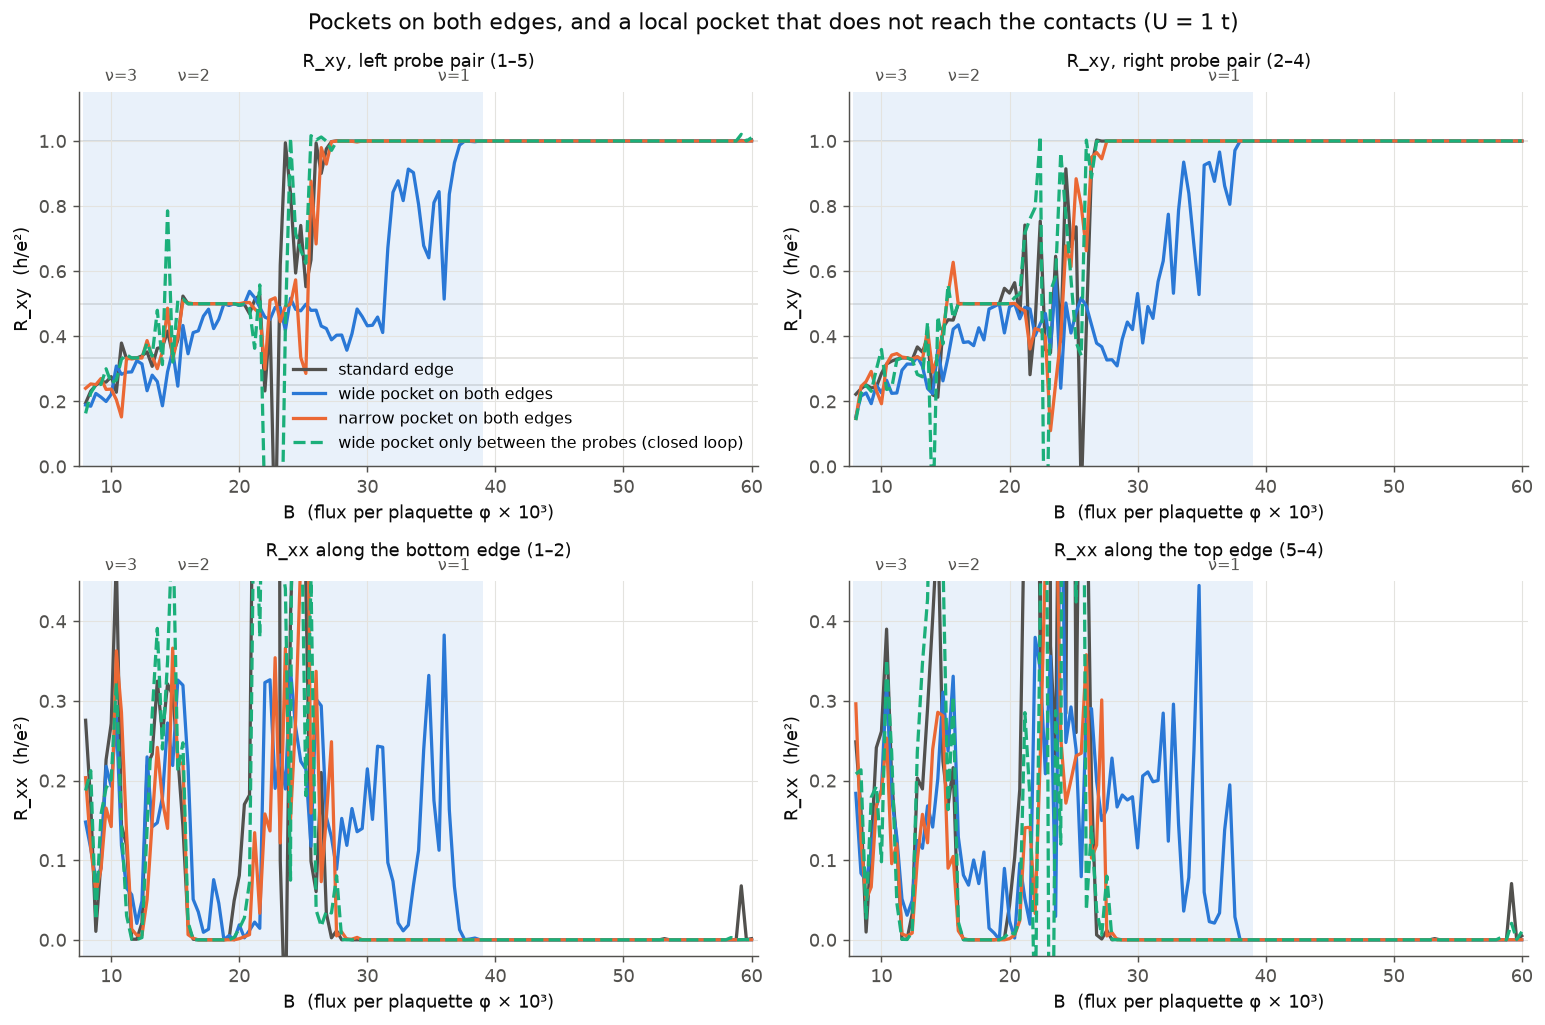
\includegraphics[width=\textwidth]{fig4_both_edges_and_local.png}
\caption{Pockets on both edges, and a local pocket that does not reach the
contacts ($U=1\,t$).}
\label{fig:both}
\end{figure}

\subsection{Where the current flows}
Fig.~\ref{fig:current} shows the current density of electrons injected from
probe 2. In the reference sample all of it follows the chiral path $2\to1$.
In the clean wide pocket a second path appears: the counter-propagating
channel carries part of the flow from probe 2 to the right, to drain 3, that
is, against the chirality. With disorder this path is weakened but
survives. In the narrow pocket with disorder only localized circulating
currents around disorder resonances remain, and the counter-propagating
path does not reach drain 3.

\begin{figure}[ht]
\centering
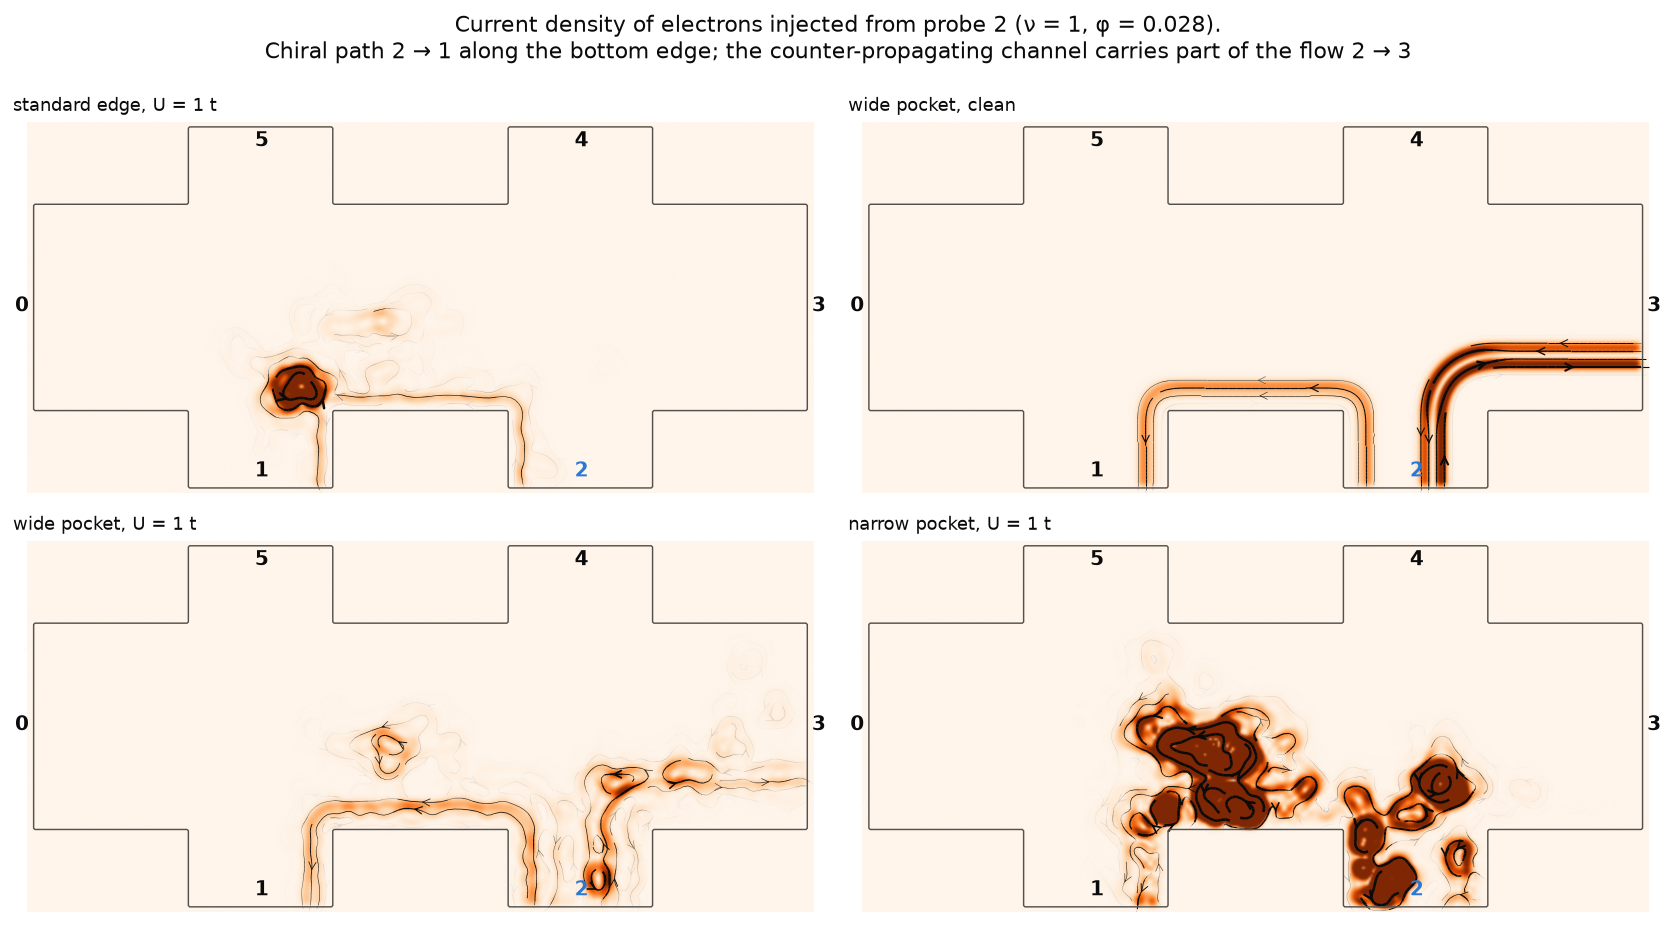
\includegraphics[width=\textwidth]{fig7_injection_from_probe2.png}
\caption{Current density of electrons injected from probe 2 ($\nu=1$,
$\varphi=0.028$). The colour scale is shared and clipped from above.}
\label{fig:current}
\end{figure}

%======================================================================
\section{The image-charge potential of~\cite{andolina}}\label{sec:image}

\subsection{What Ref.~\cite{andolina} claims}
In a single-electron model, $U_\text{im}=-e^2/(8\pi\varepsilon|x-d_\text{edge}|)$
plus a steep confining potential produce a well at the edge. The energy
scale is the \emph{backscattering energy}
\begin{equation}
\Gamma_\ell=\lB\sqrt{\ell+1}\;\partial_xU_\text{im}\big|_\text{edge}
=\frac{e^2}{8\pi\varepsilon}\frac{\lB\sqrt{\ell+1}}{d_\text{edge}^2},
\end{equation}
the potential drop across the cyclotron orbit. When $\EF$ is within
$\sim\Gamma_\ell$ of the pocket bottom, the counter-propagating states are
at most $\sim\lB\sqrt{\ell+1}$ apart, electrons backscatter, and the
two-terminal $G(\EF)$ is not quantized. The Kwant calculations
of~\cite{andolina} (Harper--Hofstadter model, field-free leads) give only
the two-terminal conductance; the Zeeman (odd) plateaus turn out to be the
most fragile.

\subsection{Parameters}
We use the profile~\eqref{eq:img} with $d_\text{edge}=18\,a\approx8\,\lB$
at $\nu=1$ (the same ratio $d_\text{edge}/\lB$ as the estimate
of~\cite{andolina} for the experiment) and $E_\text{img}=9$. The well is
then $0.22\,t\approx0.58\,\hw$ deep and $\Gamma_0=0.036\,t\approx0.1\,\hw$
at $\varphi=0.03$: between the ``realistic'' estimate of~\cite{andolina}
($\Gamma_0/\hw\sim0.02$) and the values $0.2$--$0.4$ used in the figures of
that paper. The pocket is on the bottom edge only, including the bottom
probes and the leads.

In this pocket the separation of the pair is not fixed by a window width
but grows with energy (Fig.~\ref{fig:imgprof}, right). Near the pocket
bottom the partners overlap ($O>0.3$ within $\approx\Gamma_0$ of the
bottom); higher up they move apart to 10--15~$\lB$. One pocket therefore
contains both regimes of Sec.~\ref{sec:rect}, at different $\EF$ or $B$. In
addition, the inner partner sits on the gentle $1/d$ tail, and its velocity
is 4--5 times lower than in the rectangular pocket ($v\approx0.04$--$0.05$
versus $0.16$--$0.21$ in units of $ta/\hbar$), so disorder backscatters it
even when the pair is noticeably separated.

\begin{figure}[ht]
\centering
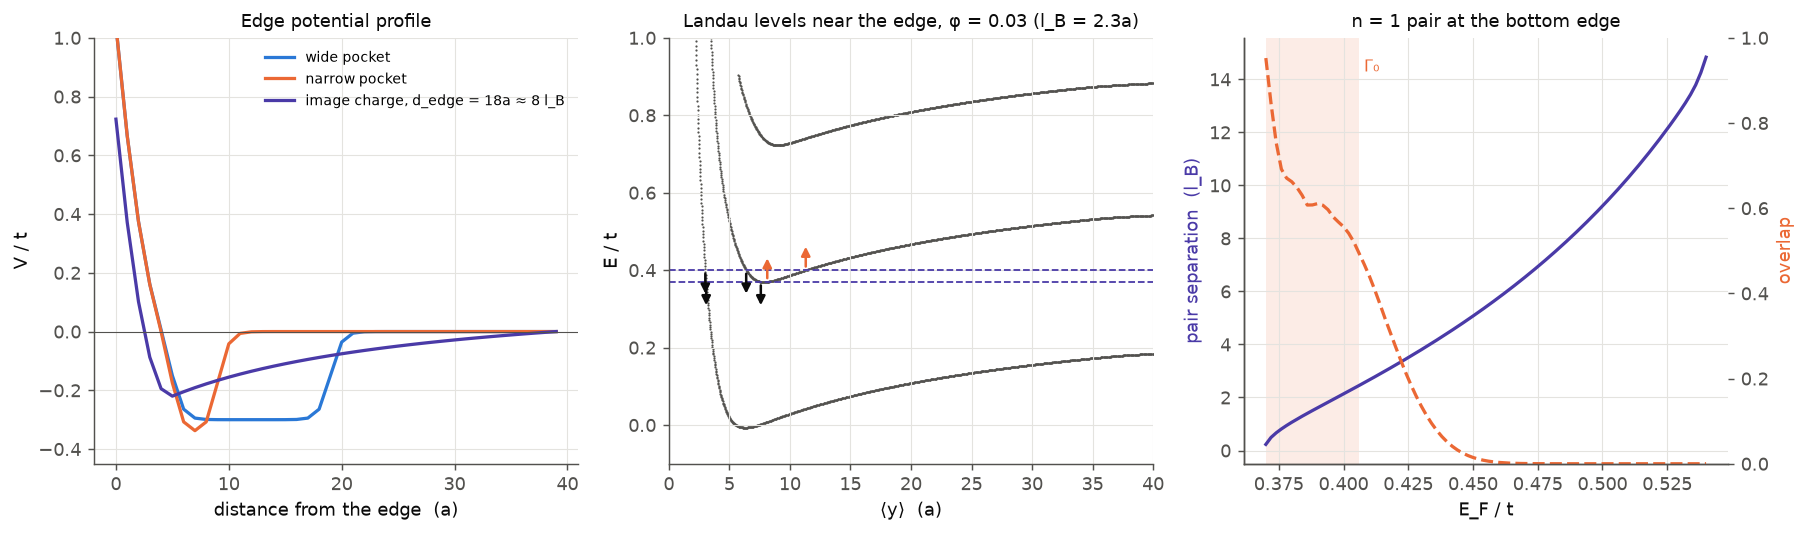
\includegraphics[width=\textwidth]{fig8_image_profile.png}
\caption{Left: edge profiles (wide and narrow pockets, image-charge
potential). Centre: bent Landau levels near the edge with the image-charge
potential at $\varphi=0.03$, and the modes at two Fermi energies. Right:
separation and overlap of the $n=1$ pair as a function of $\EF$; the shading
marks the window $\Gamma_0$ above the pocket bottom.}
\label{fig:imgprof}
\end{figure}

\subsection{Field sweep}
At $\EF=0.4\,t$ (Fig.~\ref{fig:imgB}):
\begin{itemize}
\item Without disorder we again get exactly Table~\ref{tab:lb} with $\tb=1$
  throughout the window where the pair exists: at $\nu=1$
  $\Rxy^{(1\text{--}5)}=1/2$, $\Rxy^{(2\text{--}4)}=3/4$, $\Rxx^\botm=1/4$;
  at $\nu=2$ and 3, $1/3,\,4/9,\,1/9$ and $1/4,\,5/16,\,1/16$. Note that
  $\Rxy^{(1\text{--}5)}=1/(\nu+1)$ looks like a continuation of the
  neighbouring plateau; only $\Rxy^{(2\text{--}4)}$ and $\Rxx$ of the bottom
  edge give the pair away.
\item With disorder, on the high-field part of the window
  ($\varphi\approx0.029$--$0.032$, overlapping pair), $\tb\le0.11$ (mean over
  segments) and $\Rxy^{(1\text{--}5)}=0.86$--$1.00$. On the low-field part
  (separated pair) $\Rxy^{(1\text{--}5)}$ drops to 0.44--0.70 and
  $\Rxx^\botm$ rises to 0.33. This window, however, coincides with the
  $2\to1$ bulk transition of the reference, so below we repeat the
  comparison at fixed field.
\end{itemize}

\begin{figure}[ht]
\centering
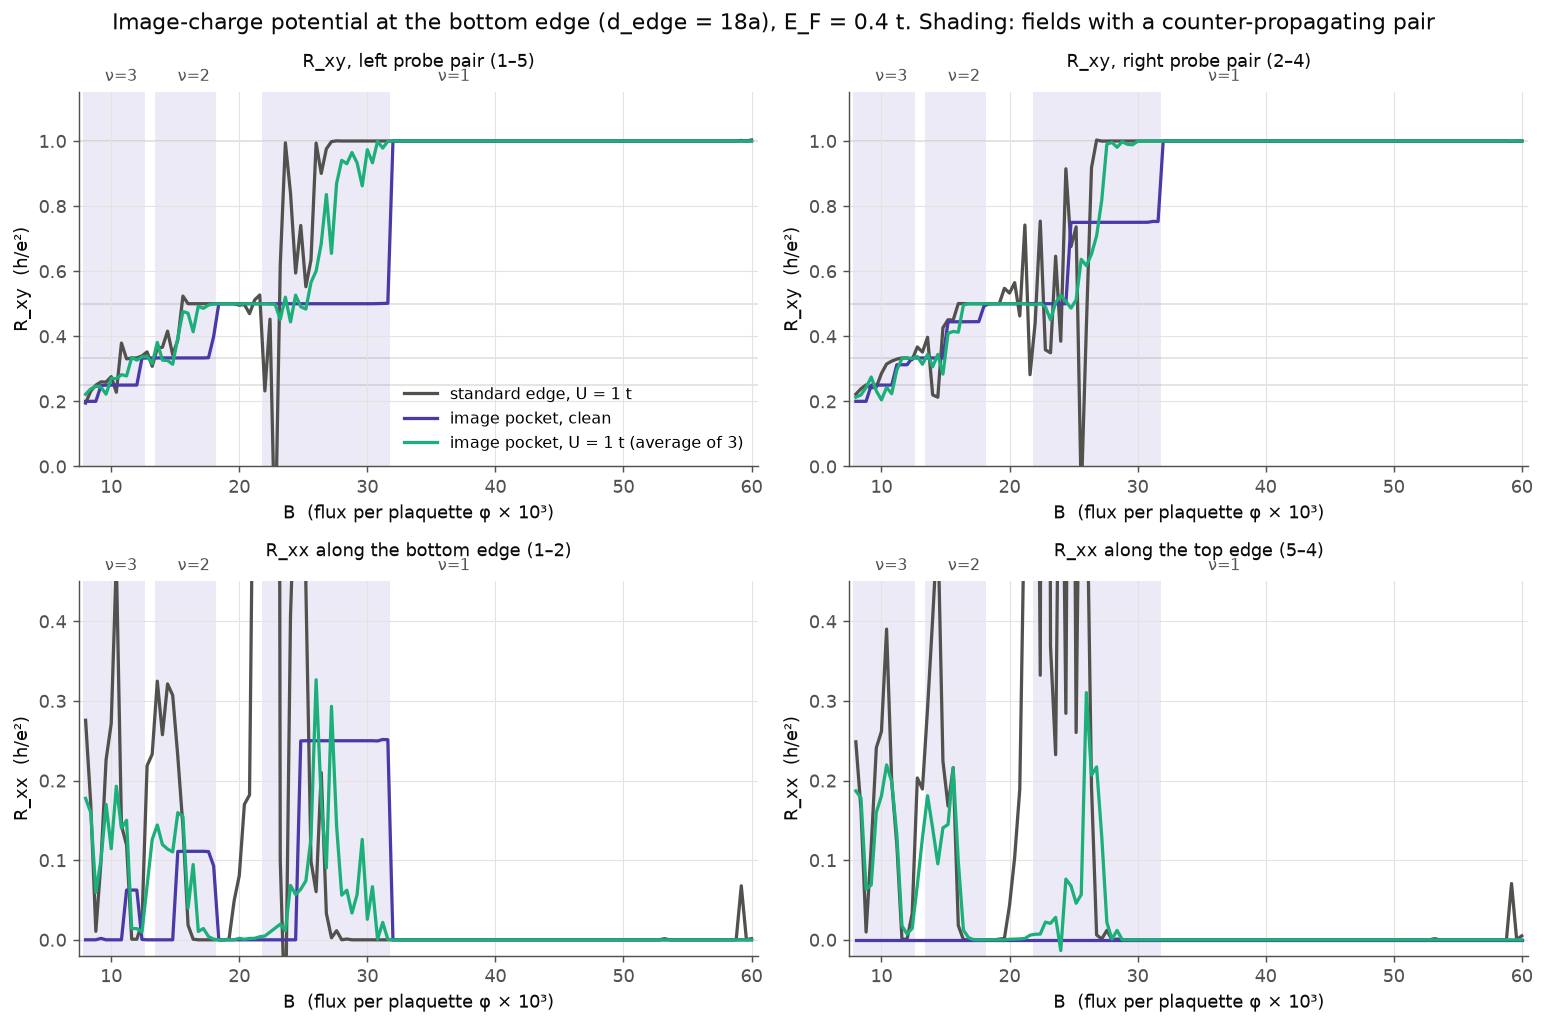
\includegraphics[width=\textwidth]{fig9_image_B_sweep.png}
\caption{Image-charge potential at the bottom edge, field sweep at
$\EF=0.4\,t$. Shading: fields with a counter-propagating pair.}
\label{fig:imgB}
\end{figure}

\subsection{Sweep of $\EF$ at fixed field (the protocol of~\cite{andolina})}
At $\varphi=0.03$ the same sample is computed both as a Hall bar and as a
plain two-terminal bar (Fig.~\ref{fig:imgEF}, Table~\ref{tab:ef}). Values
with disorder are averaged over three realizations.

\begin{table}[ht]
\centering
\caption{$\EF$ sweep at $\varphi=0.03$, image-charge potential, $U=1\,t$.
At $\EF<0.19$ the bulk is empty, the top probes carry no channels, and the
Hall bar cannot be measured; only $G_\text{2t}$ remains.}
\label{tab:ef}
\resizebox{\textwidth}{!}{%
\begin{tabular}{@{}lllccc@{}}
\toprule
$\EF/t$ & pair & $G_\text{2t}$, $e^2/h$ & $\Rxy^{(1\text{--}5)}$ & $\Rxx^\botm$ & reference $\Rxy$, $\Rxx$\\
\midrule
0.000--0.048 ($\nu=0$) & 0.8--3.2 $\lB$ & $\le0.003$ (clean: 1) & --- & --- & $G_\text{2t}=0$\\
0.052--0.12 ($\nu=0$) & 3.4--7.9 $\lB$ & $0.07\to0.98$ & --- & --- & $G_\text{2t}=0$\\
0.372--0.412 ($\nu=1$) & 0.5--2.8 $\lB$, $O$=0.85--0.41 & 1.000 & 0.97--1.00$^a$ & $\le0.03^a$ & 1, 0\\
0.416--0.432 ($\nu=1$) & 3.0--3.9 $\lB$, $O$=0.34--0.11 & 0.986--1.000 & 0.81--0.91 & 0.09--0.19 & 1, $\le10^{-4}$\\
0.436--0.448 ($\nu=1$) & 4.2--4.9 $\lB$, $O\le0.08$ & 0.89--1.035 & 0.73--0.92 & 0.09--0.29 & 1, $\le0.016$\\
0.372--0.49, $U=0$ & & 2 & 0.50 & 0.25 & \\
\bottomrule
\end{tabular}}\\[2pt]
{\footnotesize $^a$ one point: $\Rxy=0.88$, $\Rxx=0.12$.}
\end{table}

\begin{itemize}
\item \textbf{The $\nu=0$ window is the analogue of Figs.~3 and S1
  of~\cite{andolina}.} Above the pocket bottom $G_\text{2t}<1$ and grows
  towards 1 as the pair separates. In our long sample with strong disorder
  this window is wider than $\Gamma_0$, and inside it $G_\text{2t}=0$ (the
  counter-propagating channel is fully localized) rather than partially
  suppressed.
\item \textbf{The $\nu=1$ window is the main difference between the two
  measurements.} While the pair overlaps it is localized, and both
  measurements are quantized. Once the partners are 3--4~$\lB$ apart, the
  Hall bar is already clearly non-quantized ($\Rxx^\botm=0.09$--$0.19$, with
  the reference quantized to $10^{-4}$), while $G_\text{2t}$ is still
  0.986--1.000. In individual realizations $\Rxx^\botm$ reaches 0.4 and
  $\tb$ of individual segments reaches 0.55.
\item From $\EF\approx0.436$ the reference starts to deviate from
  quantization, and at $\EF\ge0.452$ its bulk transition begins, so the
  comparison is no longer meaningful.
\end{itemize}

\begin{figure}[ht]
\centering
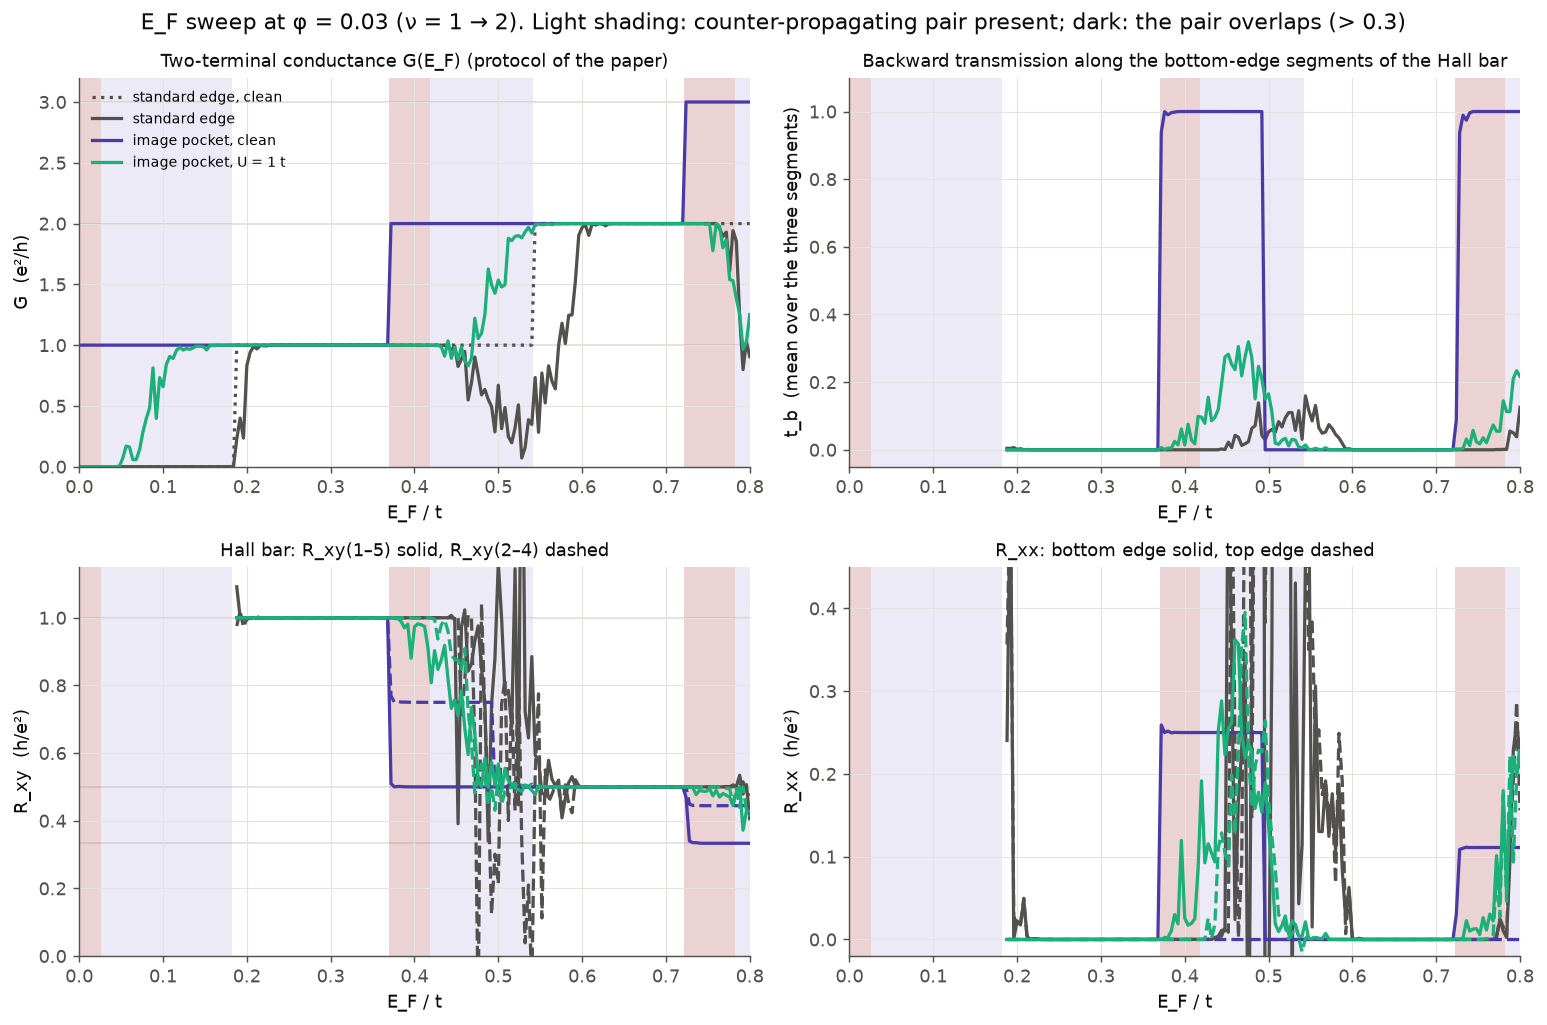
\includegraphics[width=\textwidth]{fig10_image_EF_sweep.png}
\caption{$\EF$ sweep at $\varphi=0.03$. Light shading: counter-propagating
pair present; dark: the pair overlaps ($O>0.3$). Top left: two-terminal
conductance of the plain bar (protocol of~\cite{andolina}); top right:
$\tb$ averaged over the three bottom-edge segments of the Hall bar; bottom:
Hall-bar resistances.}
\label{fig:imgEF}
\end{figure}

%======================================================================
\section{Interpretation and comparison with~\cite{andolina,ciuti}}

\begin{enumerate}
\item \textbf{Same physics, different observables.} By~\eqref{eq:g2t} the
  two-terminal conductance is an integer both for $\tb=0$ (as if there were
  no pair) and for $\tb=1$ (the ballistic pair counts as one more channel);
  only an intermediate $\tb$ is visible. In the Hall bar, $\tb$ of each
  segment between neighbouring contacts produces $\Rxx$ and a difference of
  Hall voltages, and $\tb=1$ gives the \emph{largest} deviation. The
  ``breakdown of quantization'' of~\cite{andolina} (intermediate $\tb$ near
  the pocket bottom) and the ``protection of quantization by
  backscattering'' of Sec.~\ref{sec:rect} are two ends of the same
  dependence of $\tb$ on the pair separation. Which one is observed depends
  on the edge length between contacts, the disorder strength and the way
  the measurement is done.
\item \textbf{The plateau labels differ.} In~\cite{andolina}
  ``quantized'' means $G=\nu+1$ above the pocket bottom (the ballistic pair
  counted as a channel), and breakdown means $G<\nu+1$ within the window
  $\Gamma_\ell$. For a Hall bar with bulk filling $\nu$, quantization means
  $\Rxy=h/\nu e^2$ and $\Rxx=0$, i.e.\ $\tb=0$.
\item \textbf{The four-terminal measurement is more sensitive.} A segment
  between probes (60--70~$a$) is shorter than the whole edge (300~$a$), and
  $\tb\sim e^{-L/\xi}$ is larger on it. At $\EF=0.416$--$0.432$
  $G_\text{2t}$ differs from 1 by at most 0.015, while $\Rxx^\botm$ of the
  same sample is 0.09--0.19~$\he$.
\item \textbf{The comment~\cite{ciuti}.} We do not test its first objection
  (no pocket because of the donor background, Fermi-level pinning at the
  etched surface and a surface-state capacitance $\gg\varepsilon_0/d$): all
  our conclusions are conditional, \emph{if} a pocket exists. The second
  objection (the paper does not compute $\Rxx$ and $\Rxy$) is answered
  directly by our calculation: in a six-terminal Hall bar such a pocket gives
  $\Rxx\neq0$ \emph{only along the edge next to the metal}, different $\Rxy$
  on the two probe pairs (their difference equals $\Rxx$ of that edge), and
  deviations only on the low-field side of the plateaus. This distinguishes
  the mechanism from a bulk one (for instance vacuum-induced), for which
  $\Rxx$ appears along both edges.
\item \textbf{What of~\cite{andolina} is missing here:} spin and the Zeeman
  plateaus, finite temperature, fixed particle number. The leads in the code
  of~\cite{andolina} have neither field nor pocket, ours have both; in both
  cases the counter-propagating channel ends in a contact, so this does not
  affect the conclusion.
\end{enumerate}

%======================================================================
\section{Conclusions and experimental signatures}

\begin{enumerate}
\item A counter-propagating partner of the chiral channel appears when the
  edge hosts a pocket about as deep as the distance from $\EF$ to the next
  Landau level. This happens on the low-field side of every plateau.
\item The intuition that ``backscattering on one edge should not spoil the
  Hall response'' is correct, and in a stronger form: backscattering inside
  an edge cannot break quantization, it protects it. Everything that happens
  inside an edge between two contacts reduces to $\tb$, and quantization is
  broken only for $\tb\neq0$.
\item Deviations of $\Rxy$ from $h/\nu e^2$ and $\Rxx\neq0$ appear when the
  counter-propagating channel is \emph{not} backscattered (the partners do
  not overlap) \emph{and} reaches ohmic contacts. The bulk $\sigma_{xy}$
  stays $\nu e^2/h$: this is an effect of the contacts and the geometry, not
  a breakdown of topology.
\item With the image-charge potential of~\cite{andolina} the picture is the
  same. As the partners separate, $\Rxx$ and the difference of Hall voltages
  appear in the Hall bar before the two-terminal $G$ deviates.
\end{enumerate}
Experimental signatures of the scenario:
\begin{itemize}
\item $\Rxx\neq0$ only along the edge that has the pocket (the metal);
\item the Hall voltages on different probe pairs differ by exactly $\Rxx$
  of that edge;
\item the effect is concentrated on the low-field side of the plateaus and
  disappears if the pocket does not reach the contacts;
\item a two-terminal measurement may barely show it.
\end{itemize}

%======================================================================
\section{Limitations}
\begin{itemize}
\item The model is single-particle and coherent: there is no
  electron--electron interaction, no edge reconstruction and no inelastic
  equilibration between channels. Equilibration over lengths longer than
  the equilibration length also gives $\tb\to0$ (as for $\nu=2/3$).
\item The pocket is put in by hand; whether it forms in the self-consistent
  electrostatics of a real mesa~\cite{ciuti,chklovskii} is not addressed
  here.
\item The sample is mesoscopic ($L\approx125\,\lB$), so the transitions
  between plateaus fluctuate strongly. The main curves are averaged over
  three disorder realizations, some curves are a single realization.
\item The pocket parameters are chosen for clarity, not fitted to a
  particular experiment.
\end{itemize}

%======================================================================
\appendix
\section{Reproducibility}
{\raggedright Code and data are in the \texttt{qhe\_pockets/} directory of the
repository: \texttt{model.py} (geometry, potentials, transport),
\texttt{lb.py} (Landauer--Büttiker model), \texttt{edge\_modes.py} (ribbon
modes), \texttt{run\_sweeps.py}, \texttt{width\_sweep.py},
\texttt{image\_sweeps.py} (calculations), \texttt{plots.py},
\texttt{plots\_image.py} (figures), \texttt{plots\_en.py} (English figures).\par}
\begin{verbatim}
conda install -c conda-forge kwant matplotlib scipy
OMP_NUM_THREADS=1 python run_sweeps.py    # ~1 h on 4 cores
OMP_NUM_THREADS=1 python width_sweep.py   # ~20 min
OMP_NUM_THREADS=1 python image_sweeps.py  # ~20 min
python plots.py && python plots_image.py && python plots_en.py
\end{verbatim}
A note on the field calibration: \texttt{kwant.physics.magnetic\_gauge}
needs $B=2\varphi$ to produce $\varphi$ flux quanta per plaquette (checked
for Kwant 1.5).

\begin{thebibliography}{9}
\bibitem{andolina} G.~M.~Andolina, Z.~Bacciconi, A.~Nardin, M.~Schirò,
  P.~Rabl, D.~De~Bernardis, \emph{Electrostatics-induced breakdown of the
  integer quantum Hall effect in cavity QED},
  \href{https://arxiv.org/abs/2511.04744}{arXiv:2511.04744}.
\bibitem{ciuti} C.~Ciuti, G.~Scalari, J.~Faist, \emph{Comment on
  ``Electrostatics-induced breakdown of the integer quantum Hall effect in
  cavity QED''}, \href{https://arxiv.org/abs/2601.14974}{arXiv:2601.14974}.
\bibitem{appugliese} F.~Appugliese \emph{et al.}, \emph{Breakdown of
  topological protection by cavity vacuum fields in the integer quantum Hall
  effect}, Science \textbf{375}, 1030 (2022).
\bibitem{buttiker} M.~Büttiker, \emph{Absence of backscattering in the
  quantum Hall effect in multiprobe conductors}, Phys.\ Rev.\ B \textbf{38},
  9375 (1988).
\bibitem{kwant} C.~W.~Groth, M.~Wimmer, A.~R.~Akhmerov, X.~Waintal,
  \emph{Kwant: a software package for quantum transport}, New J.\ Phys.\
  \textbf{16}, 063065 (2014).
\bibitem{chklovskii} D.~B.~Chklovskii, B.~I.~Shklovskii, L.~I.~Glazman,
  \emph{Electrostatics of edge channels}, Phys.\ Rev.\ B \textbf{46}, 4026
  (1992).
\end{thebibliography}

\end{document}
